% !TEX encoding = UTF-8
\documentclass{hitgsrep}
\usepackage{graphicx}
\usepackage{amsmath}
\usepackage{physics}
\usepackage{caption}
\usepackage[labelformat=simple]{subcaption}
\usepackage[section]{placeins}
\usepackage{tikz}
\usepackage{makecell}
\usepackage[outputdir={out}]{minted}% 代码高亮,需要Pygments
\usepackage{url}

\usetikzlibrary{shapes,arrows,chains,fit,positioning,backgrounds}

\hitgsrepset{
    author={李,陈,卢,李,李}, % 学生姓名
    studentid={19SXXXXXX}, % 学号
    studentcat={必修}, % 学生类别
    course={数字图像处理}, % 考核科目
    affiliation={仪器科学与工程学院}, % 学生所在院(系)
    discipline={仪器科学与技术}, % 学生所在学科
%    year={\the\year}, % 年份(不填根据当前时间自动生成)
%    semester={秋}, % 学期(不填根据当前时间自动生成)
}

\ctexset{
    section/format=\Large\bfseries
}

% C++代码高亮
\newmintedfile[cppfile]{cpp}{linenos,mathescape,fontsize=\footnotesize}

\renewcommand\thesubfigure{(\alph{subfigure})} % 得到“图 1(a)”形式的引用

% \newcommand{\todo}{{\emph{待完善}\par}}

\begin{document}
\maketitle

\section{题目}

局部统计特征增强

并与全局直方图均衡化对比,用钨丝灰度图。

\section{数学原理}

\subsection{全局直方图均衡化}

考虑连续灰度值,并用$r$表示待处理图像的灰度。考虑灰度映射
\begin{equation}
    s=T(r)\qc{0\le r\le L-1}
\end{equation}
满足
\begin{enumerate}
    \item $T(r)$在区间$[0,L-1]$上单调递增;
    \item 当$0\le r\le L-1$时,$0\le T(r)\le L-1$。
\end{enumerate}

一幅图像的灰度级可以看作是$[0,L-1]$范围内的随机变量,其概率密度函数(PDF)刻画了灰度分布的基本形态。
令$p_r(r)$和$p_s(s)$分别为随机变量$r$和$s$的概率密度函数。
由概率论知识可以知道,由于$T(r)$的单调性,代表相同范围的累积分布函数(CDF)应该相等
\begin{equation}\label{eq:cdf-eq}
    \int_{0}^{s}p_s(s')\dd{s'}=\int_{0}^{r}p_r(r')\dd{r'}
\end{equation}

所谓直方图均衡化,即通过变换将原始图像的灰度级分布变换到全部灰度范围上的均匀分布,从而增强图像的对比度。
这一目的亦即,寻找$s=T(r)$使
\begin{equation}\label{eq:hist-eql-target}
    p_s(s)=\frac{1}{L-1}
\end{equation}

将式~\eqref{eq:hist-eql-target} 代入式~\eqref{eq:cdf-eq},即可得到
\begin{equation}\label{eq:hist-eql-cont}
    s=T(r)=(L-1)\int_0^r p_r(r')\dd{r'}
\end{equation}

为了对数字图像进行处理,必须引入离散形式的公式。
当灰度级是离散值的时候,可以用频数近似代替概率值,即
\begin{equation}
    p_r\qty(r_k)=n_k/n\qc{k=0,1,\cdots,L-1}
\end{equation}
其中,$n$为图像总像素数,$n_k$是灰度为$r_k$的像素个数,$L$是图像可能的灰度级数目。
从而可以给出式~\eqref{eq:hist-eql-cont} 的离散形式
\begin{equation}
    s_k=T\qty(r_k)=(L-1)\sum_{j=0}^k p_r(r_j)=\frac{L-1}{n}\sum_{j=0}^k n_j\qc{k=0,1,\cdots,L-1}
\end{equation}
变换$T(r_k)$即\emph{直方图均衡化}。

\subsection{基于局部统计特征的增强}

在某些情况下,我们需要在增强暗色区域的同时尽可能保持明亮区域不变,因为明亮区域并不需要增强。
为了解决这类问题,需要一种能分辨亮区域和暗区域的不同,并只增强暗区域的方法。

为了表征一个点$(x,y)$局部的亮暗,可以用将局部灰度平均值$m_{S_{x,y}}$同整个图像的全局灰度平均值$m_G$进行比较:
如果$m_{S_{x,y}}\le k_0m_G$,其中$k_0$是一个小于$1$的正的常数,那么我们将把点$(x,y)$处的像素考虑为处理的候选点。

因为我们的目标在于增强低对比度的感兴趣区域,所以还需要一种方法来判定一个区域是否可以作为增强的候选点。
图像或者区域的对比度可以用标准差来衡量。
因此,如果$\sigma_{S_{x,y}}\le k_2\sigma_G$,则认为点$(x,y)$处的像素是增强的候选点。
其中,$\sigma_G$和$\sigma_{S_{x,y}}$分别为图像全局灰度标准差和局部灰度标准差,$k_2$为正的常数。
如果我们感兴趣的区域是亮区域,则该常数应当大于$1$;相反,如果对暗区域感兴趣,则该常数应当小于$1$。

最后,我们需要限制能接受的最低的对比度值,否则该方法会试图增强标准差为零的恒定区域(如背景)。
因此,我们通过要求$k_1\sigma_G\le\sigma_{S_{x,y}}, k_1<k_2$,对局部标准差设置一个较低的阈值。
满足上述所有局部增强条件的像素点,可以通过将像素值乘以一个指定常数$E$来处理,而不满足条件的像素则保持不变。

综合上面的描述,基于局部统计特征的增强方法可以总结如下:
令$f(x,y)$表示在图像任意坐标$(x,y)$处的像素值,而令$g(x,y)$表示增强图像的对应点像素值,
则对于$x=0,1,\cdots,M-1,\,y=0,1,\cdots,N-1$,有
\begin{equation}\label{eq:local-enh}
    g(x,y)=\begin{cases}
        E\cdot f(x,y) & m_{S_{x,y}}\le m_G\,\text{且}\,k_1\sigma_G\le\sigma_{S_{x,y}}\le k_2\sigma_G\\
        f(x,y) & \text{其它}
    \end{cases}
\end{equation}

\section{算法步骤}

\subsection{直方图均衡化}

首先计算图像的直方图分布,再根据直方图求灰度的累积分布,
利用累积分布建立均衡化的变换映射,将这一变换作用到图像的每个像素上即为所求。
算法流程如图~\ref{fig:hist-eq-flowchart} 所示。

\begin{figure}[!htb]
    \centering
    \begin{tikzpicture}[%
        font=\footnotesize,
        >=triangle 60,                  % Nice arrows; your taste may be different
        start chain=going below,        % General flow is top-to-bottom
        node distance=6mm and 60mm,     % Global setup of box spacing
        every join/.style={->, draw},   % Default linetype for connecting boxes
        ]
    \tikzset{
      base/.style={draw, on chain, text centered, minimum height=4ex},
      proc/.style={base, rectangle, minimum width=10em},
      test/.style={base, diamond, aspect=2, minimum width=4em},
      term/.style={proc, rounded corners},
      coord/.style={coordinate},
      sel/.style={font=\scriptsize},
      block/.style={rectangle, minimum width=15em, draw, dashed},
    }
    % 直方图均衡化主体
    \node [term]       (in) {输入图像$f(x,y)$};
    \node [proc, join] (ht) {计算灰度直方图$p_r(r_k)$};
    \node [proc, join]      {$C(r_k)=\sum_{j=0}^k p_r(r_j)$};
    \node [proc, join]      {$T(r_k)=(L-1)\operatorname{int}[C(r_k)]$};
    \node [proc, join]      {$g(x,y)=T[f(x,y)]$};
    \node [term, join]      {输出图像$g(x,y)$};
    % 灰度直方图计算子程序
    \node [term, right=5em of in.east]      (htin)  {输入图像$f(x,y)$};
    \node [proc, join]                      (htini) {\makecell{初始化$p_r(r_k)=0$\\ $ (x,y)=(0,0)$}};
    \node [proc, join]                      (htadd) {$p_r[f(x,y)]\mathbin{{+}{=}}1/(MN)$};
    \node [test, join]                      (htnxt) {下一个像素点$(x,y)$?};
    \node [term]                            (htout) {输出直方图$p_r(r_k)$};
    \node [coord, right=3em of htnxt.east]  (htlpx) {};
    \path [*->, draw] (htnxt.south) -- node[sel,anchor=west]{遍历完成} (htout);
    \path [*-, draw] (htnxt.east) -- node[sel,anchor=south]{继续} (htlpx);
    \path [->, draw] (htlpx) |- (htadd);
    \begin{scope}[on background layer]
        \node [block,fit=(htin) (htini) (htadd) (htnxt) (htout) (htlpx), label=灰度直方图计算子程序] (htsub) {};
        \path [draw, dashed] (htsub.north west) -- (ht.north east);
        \path [draw, dashed] (htsub.south west) -- (ht.south east);
    \end{scope}
    \end{tikzpicture}
    \caption{直方图均衡化算法流程图}
    \label{fig:hist-eq-flowchart}
\end{figure}

\subsection{基于局部统计特征的增强}

首先计算图像的全局均值和标准差,然后遍历图像的每个像素点,求取其邻域内的局部均值和标准差,
然后根据式~\eqref{eq:local-enh} 决定该点是否增强以及增强的结果。
算法流程如图~\ref{fig:local-enh-flowchart} 所示。

\begin{figure}[!htb]
    \centering
    \begin{tikzpicture}[%
        font=\footnotesize,
        >=triangle 60,                  % Nice arrows; your taste may be different
        start chain=going below,        % General flow is top-to-bottom
        node distance=6mm and 60mm,     % Global setup of box spacing
        every join/.style={->, draw},   % Default linetype for connecting boxes
        ]
    \tikzset{
      base/.style={draw, on chain, text centered, minimum height=4ex},
      proc/.style={base, rectangle, minimum width=8em},
      test/.style={base, diamond, aspect=2, minimum width=4em},
      term/.style={proc, rounded corners},
      coord/.style={coordinate},
      sel/.style={font=\scriptsize},
      block/.style={rectangle, minimum width=15em, draw, dashed},
    }
    % 局部统计特征增强主体
    \node [term]                        (in)     {\makecell{输入图像$f(x,y)$以及\\ 参数$k_0,k_1,k_2,E,r$}};
    \node [proc, join]                  (glo)    {计算$m_G,\sigma_G$};
    \node [proc, join]                  (mrk)    {\makecell{选取像素点$(x,y)$\\ 及其邻域$S_{x,y}$}};
    \node [proc, join]                  (loc)    {计算$m_{S_{x,y}},\sigma_{S_{x,y}}$};
    \node [proc, join]                           {根据式~\eqref{eq:local-enh} 计算$g(x,y)$};
    \node [test, join]                  (nxt)    {下一个像素点$(x,y)$?};
    \node [term]                        (out)    {输出图像$g(x,y)$};
    \node [coord, left=3em of nxt.west] (lpx)    {};
    \path [*->, draw] (nxt.south) -- node[sel,anchor=west]{遍历完成} (out);
    \path [*-, draw] (nxt.west) -- node[sel,anchor=south]{继续} (lpx);
    \path [->, draw] (lpx) |- (mrk);
    % 计算均值与标准差
    \node [term, right=5em of in.east]      (msin)  {输入计算区域$R$};
    \node [proc, join]                      (msini) {\makecell{初始化$m_R=s_R=0$\\ 取起始点$(x,y)\in R$}};
    \node [proc, join]                      (msadd) {\makecell{$m_R\mathbin{{+}{=}}f(x,y)/(M_RN_R)$\\ $s_R\mathbin{{+}{=}}[f(x,y)]^2/(M_RN_R)$}};
    \node [test, join]                      (msnxt) {下一个像素点$(x,y)$?};
    \node [proc]                            (msstd) {$\sigma_R=\sqrt{s_R-m_R^2}$};
    \node [term, join]                      (msout) {输出$m_R,\sigma_R$};
    \node [coord, right=3em of msnxt.east]  (mslpx) {};
    \path [*->, draw] (msnxt.south) -- node[sel,anchor=west]{遍历完成} (msstd);
    \path [*-, draw] (msnxt.east) -- node[sel,anchor=south]{继续} (mslpx);
    \path [->, draw] (mslpx) |- (msadd);
    \begin{scope}[on background layer]
        \node [block,fit=(msin) (msini) (msadd) (msnxt) (msstd) (msout) (mslpx), label=均值与标准差计算子程序] (mssub) {};
        \path [draw, dashed] (mssub.north west) -- (glo.north east);
        \path [draw, dashed] (mssub.south west) -- (glo.south east);
        \path [draw, dashed] (mssub.north west) -- (loc.north east);
        \path [draw, dashed] (mssub.south west) -- (loc.south east);
    \end{scope}
    \end{tikzpicture}
    \caption{局部统计特征增强算法流程图}
    \label{fig:local-enh-flowchart}
\end{figure}

另外,值得一提的是,对于均值和标准差的计算,可以合并为一个可复用的子程序,
并根据$D(x)=E(x^2)-E(x)^2$将二者的求取放在同一个循环中进行。
使用这种方式,可能获得比直接按定义对二者分别计算更好的性能。

\section{结果分析与讨论}

\begin{figure}[!htb]
    \centering
    \subcaptionbox{原图像\label{fig:tungsten-origin}}{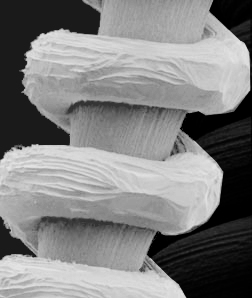
\includegraphics[width=0.3\linewidth]{tungsten.png}}\hfill
    \subcaptionbox{直方图均衡化的结果\label{fig:tungsten-global}}{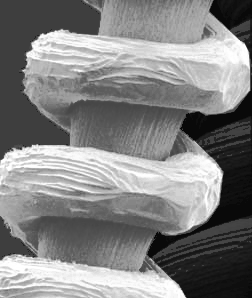
\includegraphics[width=0.3\linewidth]{tungsten-global.png}}\hfill
    \subcaptionbox{局部统计增强的结果\label{fig:tungsten-local}}{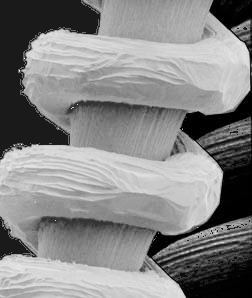
\includegraphics[width=0.3\linewidth]{tungsten-local.png}}
    \caption{放大的钨丝SEM图像及其对应增强图像}
    \label{fig:tungsten}
\end{figure}

图~\ref{fig:tungsten-origin} 显示了一根绕在支架上的钨丝的扫描电子显微镜(SEM)图像。图像中央的钨丝及其支架很清楚并很容易分析。
在该图像的右侧黑暗部分,有另一根钨丝的结构,但几乎不能察觉到,其大小与特征也难以辨认。
为了增强该图像以使暗处的钨丝也能够分辨,对图像进行了直方图均衡化处理和局部统计增强处理,
得到的结果分别如图~\ref{fig:tungsten-global} 和图~\ref{fig:tungsten-local} 所示。

\begin{figure}[!htb]
    \centering
    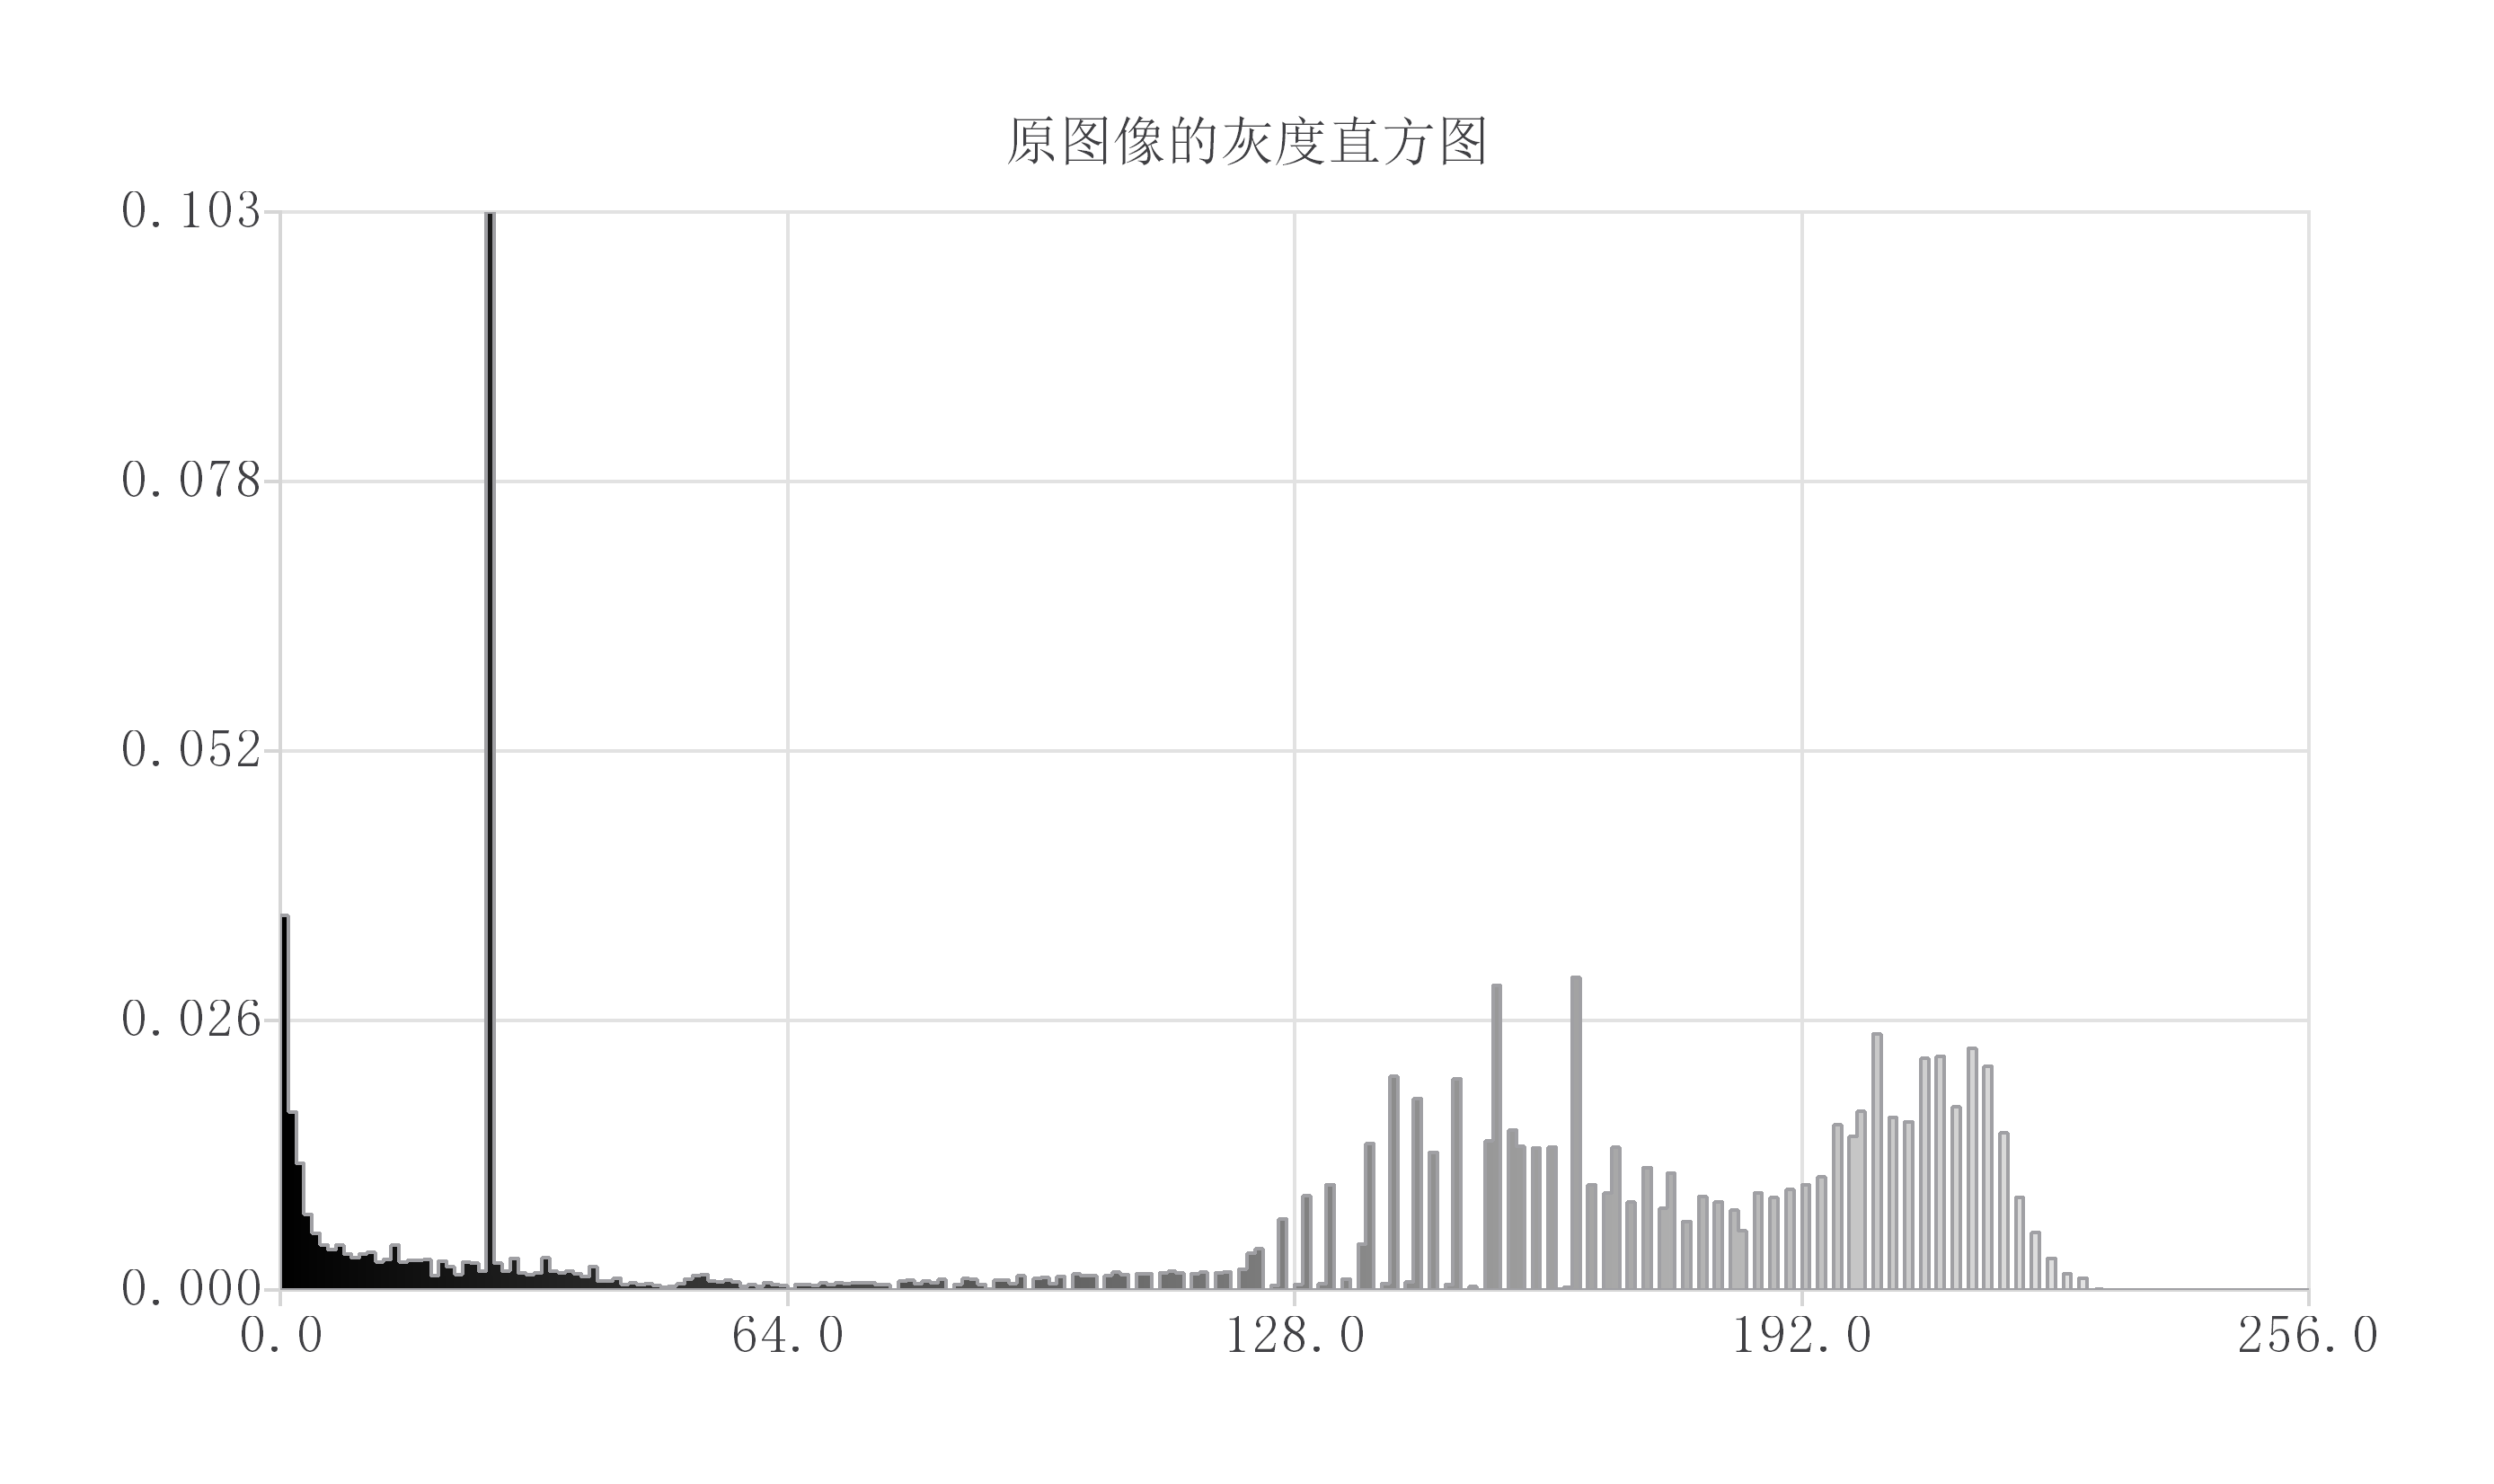
\includegraphics[width=0.8\linewidth]{tungsten-hist.png}
    \caption{原图像的灰度直方图}
    \label{fig:tungsten-origin-hist}
\end{figure}

从图~\ref{fig:tungsten-global} 中可以看到,直方图均衡化能够增强图像地对比度,补偿图像在视觉上难以区分灰度级的差别。
但它对图像的作用是在空间上是均匀的,且处理过程无法产生新的灰度级,这意味着在增强前景的同时,对大面积的均匀黑暗背景也有所增强。
通过对比图~\ref{fig:tungsten-origin-hist} 和图~\ref{fig:tungsten-global-hist} 的尖峰移动趋势可以直观的看到这种现象。
从而导致均衡化后的结果在一定程度上反而“冲淡”了人对目标和背景的辨识度。
同样,受制于这种空间上的均匀性,对于处于暗处与背景灰度相近的另一根钨丝目标,其细节的清晰度并没有明显的改善。

\begin{figure}[!htb]
    \centering
    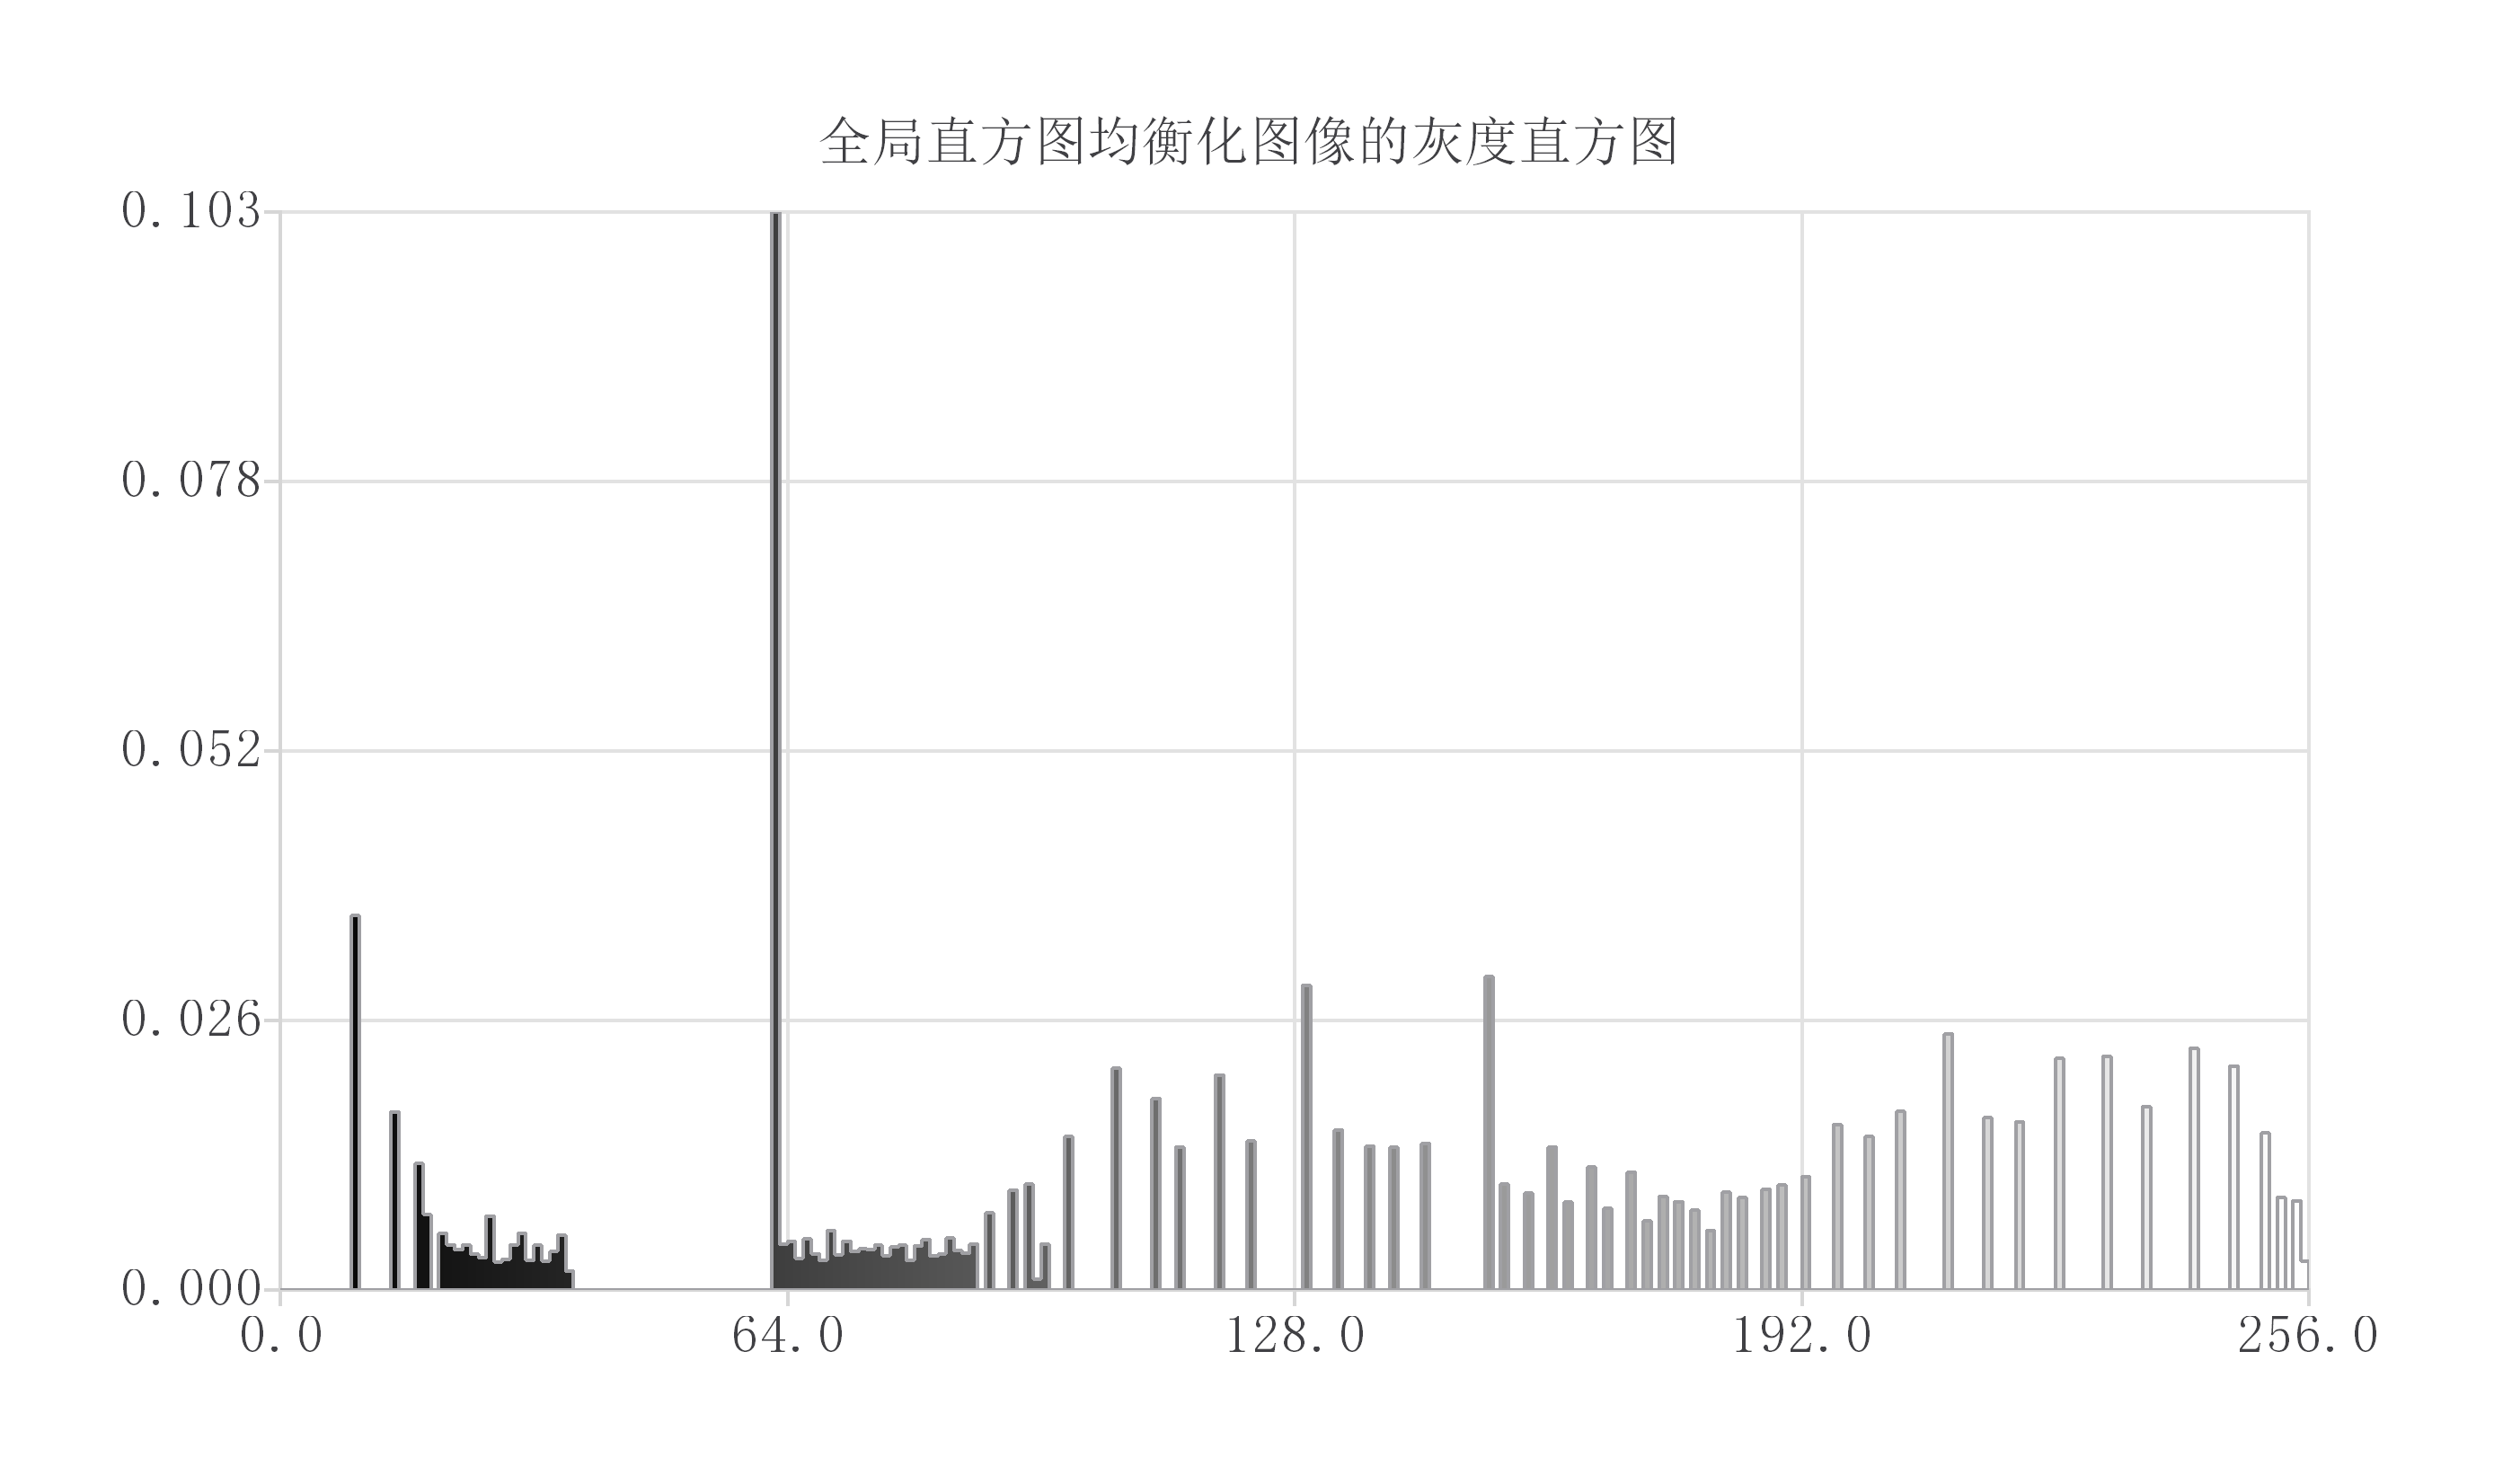
\includegraphics[width=0.8\linewidth]{tungsten-global-hist.png}
    \caption{直方图均衡化结果的灰度直方图}
    \label{fig:tungsten-global-hist}
\end{figure}

\begin{figure}[!htb]
    \centering
    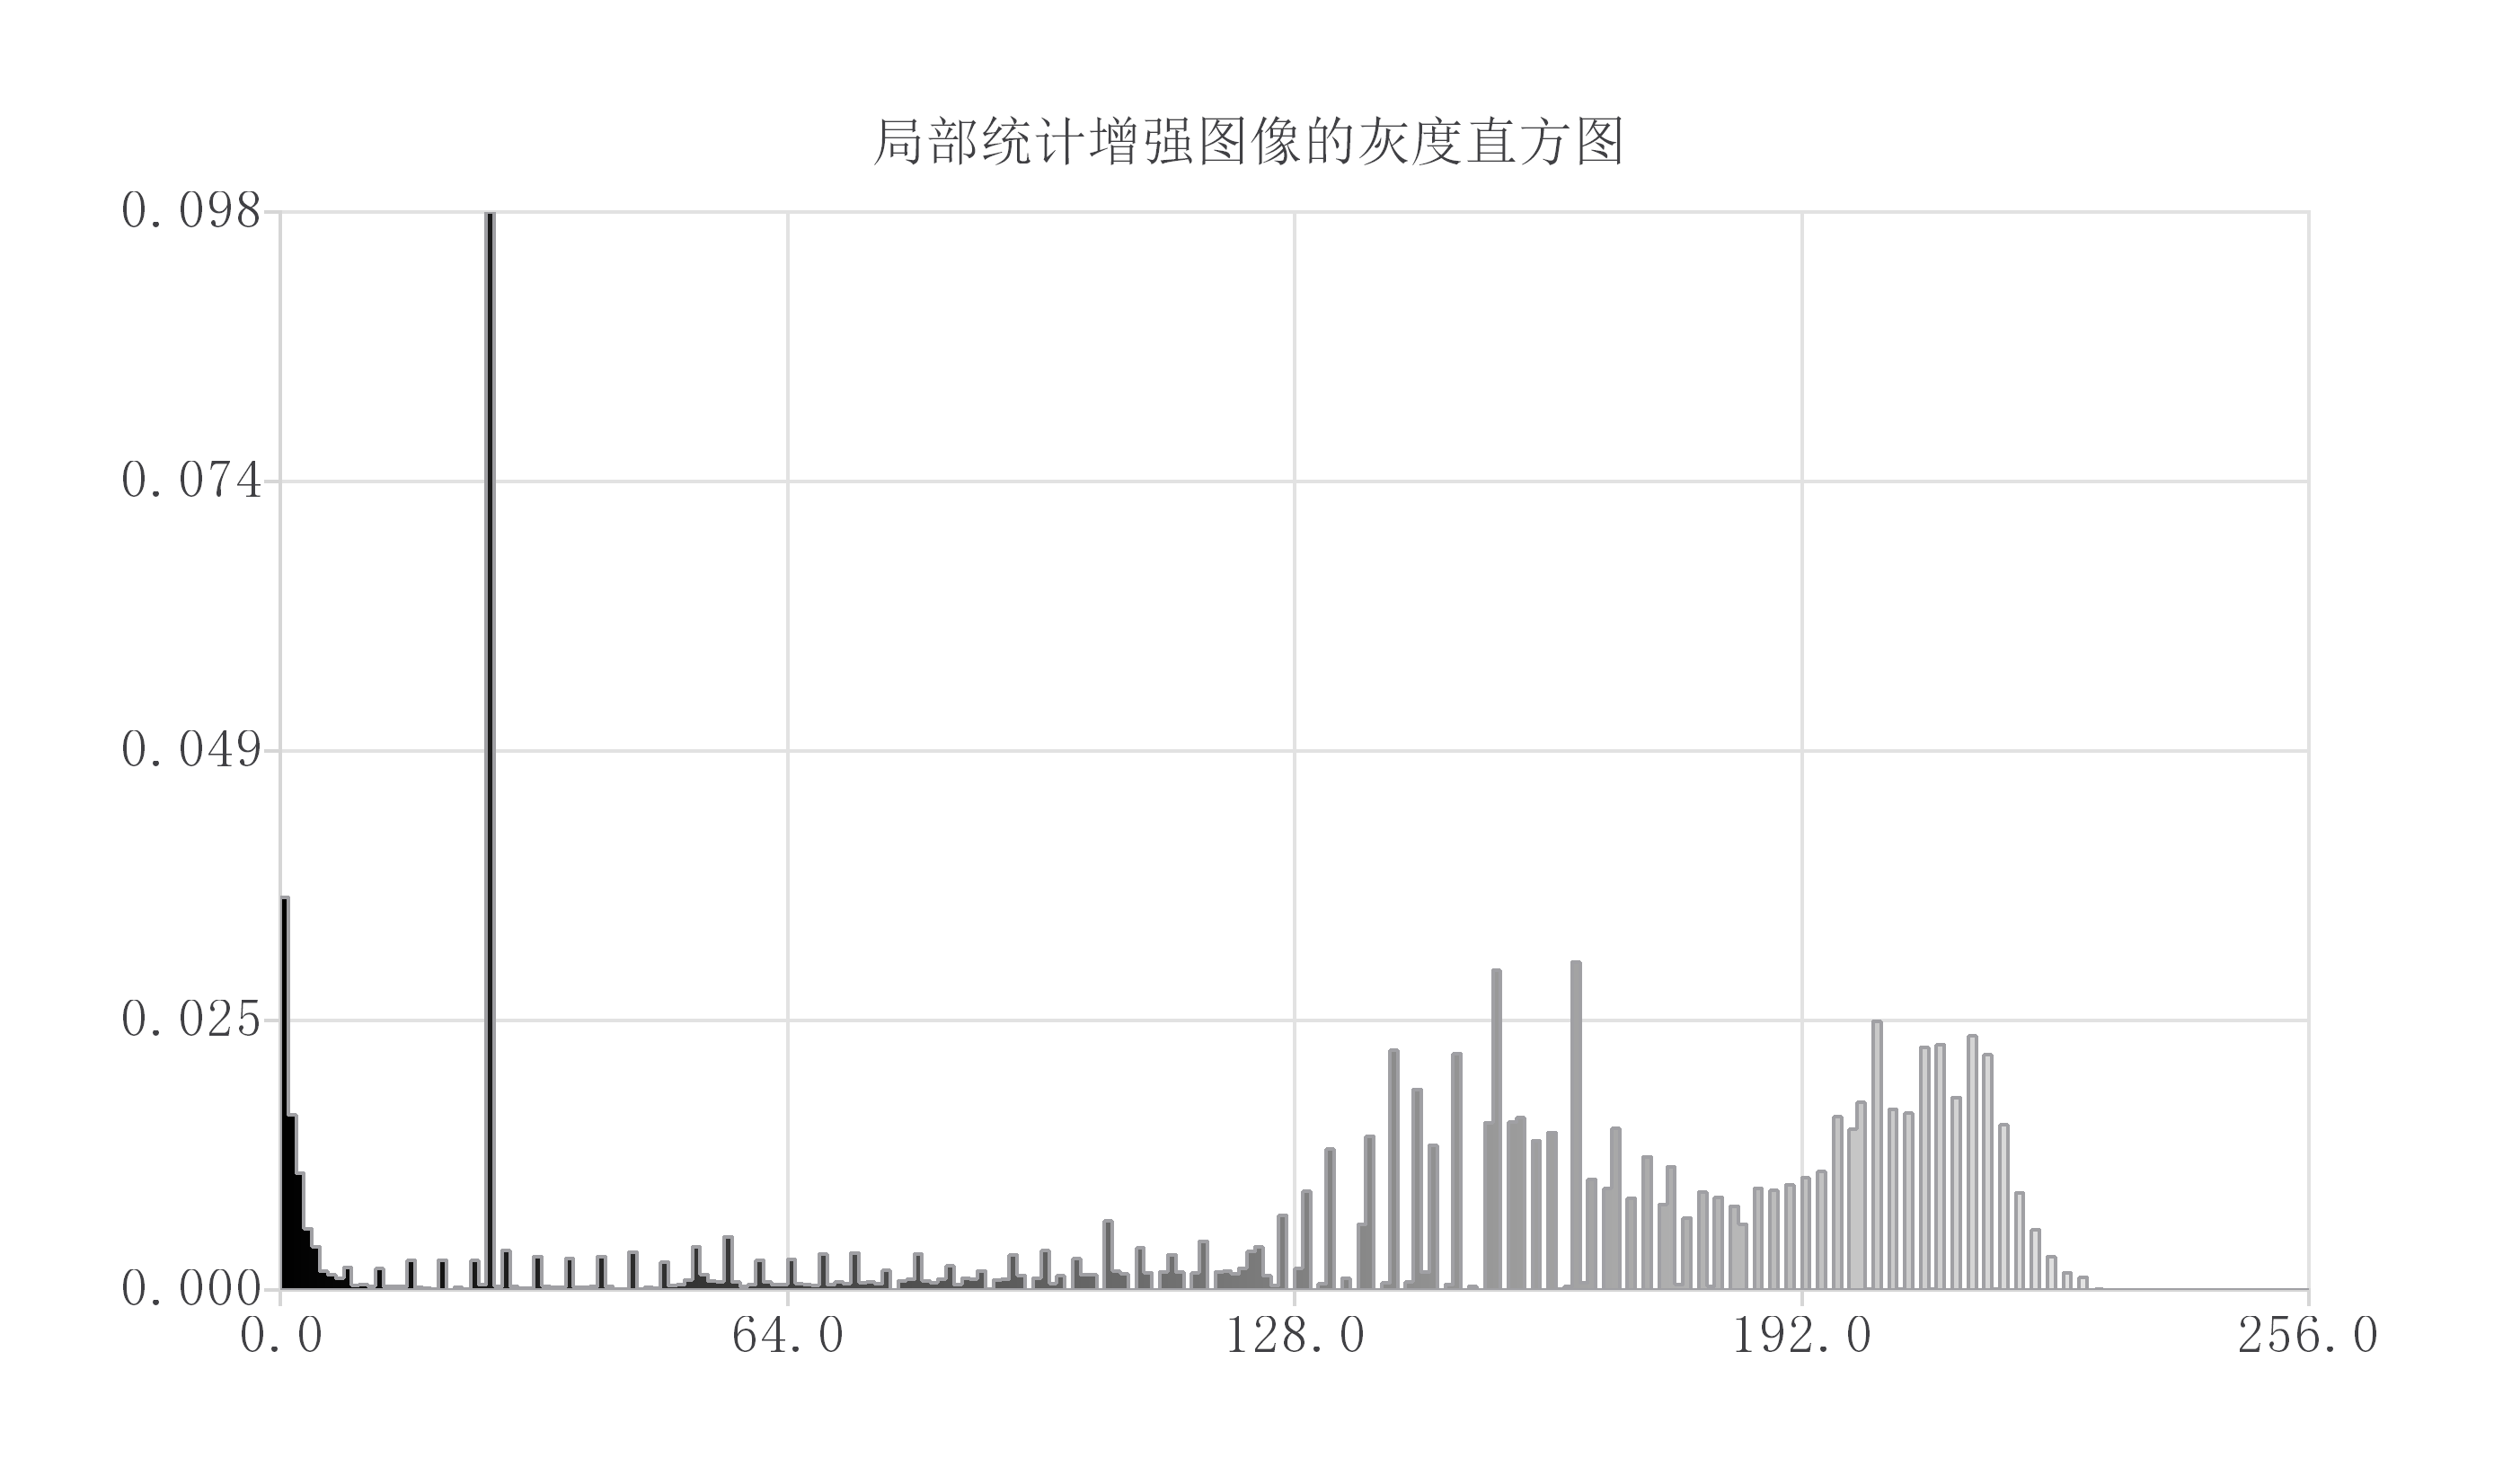
\includegraphics[width=0.8\linewidth]{tungsten-local-hist.png}
    \caption{局部统计增强结果的灰度直方图}
    \label{fig:tungsten-local-hist}
\end{figure}

图~\ref{fig:tungsten-local} 给出了基于局部统计特征增强的结果。这一方法有几个参数可以选取。
在这里使用的是 $k_0=0.4,k_1=0.02,k_2=0.4,E=4$,以及大小为 $3\times3$ 的局部区域。
这些参数一般需要通过一些试验得到,但也可以通过简单的分析估计其大致的范围。
比如 $k_0$ 选取之所以比 $50\%$ 略小,是因为我们直观上观察这副图像,
可以大致估计出我们需要增强的区域(暗处的钨丝)的灰度范围确实比全局平均灰度的一半还要略小一些。

从图~\ref{fig:tungsten-local} 中可以看到,现在暗处的钨丝脊线已经变得非常清楚,同时左侧的原本清晰的钨丝以及暗背景基本保持不变。
这表明局部统计增强能够增强暗区域的目标,同时尽可能保留亮区域的目标和背景不变。
另一方面,对比图~\ref{fig:tungsten-origin-hist} 和图~\ref{fig:tungsten-local-hist} 也可以看到局部统计增强基本不改变直方图的趋势轮廓,
不会出现全局直方图均衡化那样减弱背景和目标区分度的情况。
不过,由于目标和背景之间的边界处也会存在满足条件的对比度情况,因此局部统计增强可能导致目标边界的背景被增强,形成一道不太协调的灰色轮廓。

\appendix

\section{算法源码}

程序使用 C++ 基于 Qt 框架开发,完整的源码见 GitHub 仓库:\\
\url{https://github.com/miRoox/HIT-DigitalImageProcessing-Postgraduate}

代码仓库中也包含报告的 \LaTeX{} 源码和一个 \textsc{Matlab} 版代码。

下面只附上算法 C++ 实现的核心源码:

\noindent 头文件\textbf{algorithms.h}:

\cppfile{../DIP-src/algorithms.h}

\noindent 源文件\textbf{algorithms.cpp}:

\cppfile{../DIP-src/algorithms.cpp}

\end{document}
